\documentclass{assignment}

\course{ECO 120-04}
\name{Lucas Reddinger}
\date{Sunday 18 December 2022}
\doctitle{Assignment 14 Solutions}

\begin{document}
\RaggedRight

\beginsolutions{}

\section{Currency exchange markets}

Consider the exchange markets between the U.S.~dollar and the euro.

\begin{enumerate}

\item In the euro market, what is the price called and what are its units?

\begin{solution}
It is called an exchange rate. Its units are USD/EUR.
\end{solution}

\item In the dollar market, what are the units of its price?

\begin{solution}
Its units are EUR/USD.
\end{solution}

\item If the price of the euro increases, does the euro appreciate or depreciate?

\begin{solution}
\emph{Complete answer:} It appreciates.

This means that USD/EUR increases, so each euro is worth more dollars. It appreciates in value, relative to USD.
\end{solution}

\item If the price of the euro decreases, does the euro appreciate or depreciate?

\begin{solution}
\emph{Complete answer:} It depreciates.

This means that USD/EUR decreases, so each euro is worth less dollars. It depreciates in value, relative to USD.
\end{solution}

\item If the price of the euro increases, does the dollar appreciate or depreciate?

\begin{solution}
\emph{Complete answer:} It depreciates.

Within any two-currency exchange, if one currency appreciates, then the other depreciates. The dollar depreciates.
\end{solution}

\item If the price of the euro decreases, does the dollar appreciate or depreciate?

\begin{solution}
\emph{Complete answer:} It appreciates.

Within any two-currency exchange, if one currency depreciates, then the other appreciates. The dollar appreciates.
\end{solution}

\end{enumerate}

Suppose that France launches a successful new marketing campaign to sell more French wine in the U.S.

\begin{enumerate}[resume]

\item Please use a supply and demand model of the foreign exchange markets to illustrate the impact of this new program on the exchange rate between the dollar and the euro. Please graph both the euro market and the dollar market and clearly show the affect on each market.

\begin{solution}
Because the marketing campaign is successful, Americans want to buy more French wine. So they need to buy euros to buy French wine. So demand for euros increases. To buy these euros, Americans must supply dollars. So supply of dollars increases as well.

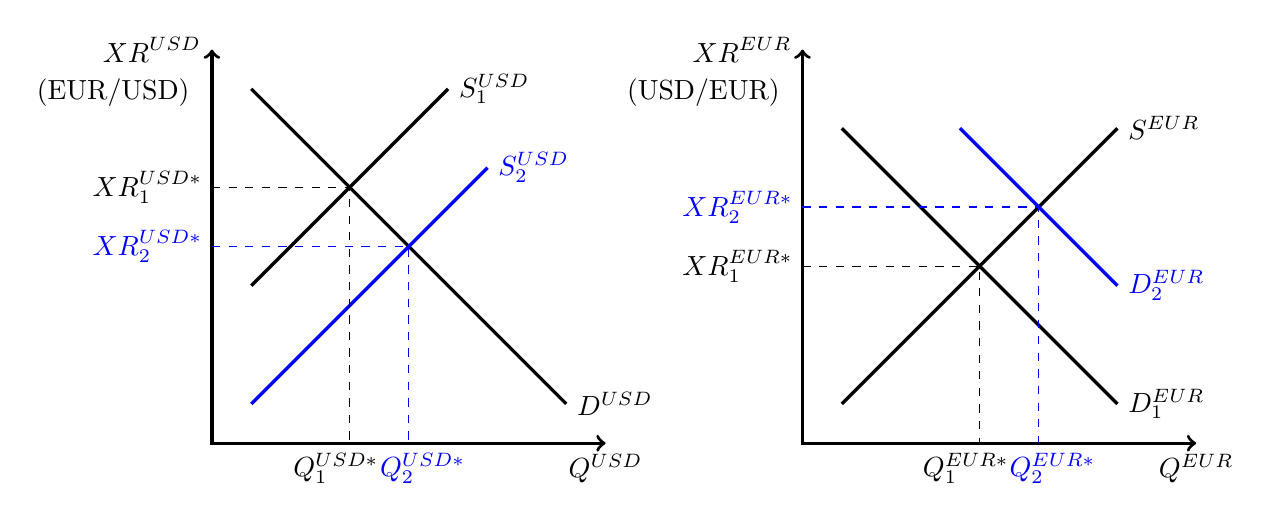
\begin{tikzpicture}[scale=0.5]
\draw[very thick,<->] (0,10) node[left,label={[align=right,xshift=-14pt,yshift=2pt]below:(EUR/USD)}]{$\text{XR}^\text{USD}$}--(0,0)--(10,0) node[below]{$Q^\text{USD}$};
\draw[very thick] (1,9)--(9,1) node[right]{$D^\text{USD}$};
\draw[very thick] (1,4)--(6,9) node[right]{$S^\text{USD}_1$};
\draw[very thick, blue] (1,1)--(7,7) node[right]{$S^\text{USD}_2$};
\draw[dashed](0,6.5) node[left] {$\text{XR}^{\text{USD}*}_1$} --(3.5,6.5)--(3.5,0) node[below,xshift=-5pt] {$Q^{\text{USD}*}_1$};
\draw[dashed, blue](0,5) node[left] {$\text{XR}^{\text{USD}*}_2$} --(5,5)--(5,0) node[below,xshift=5pt] {$Q^{\text{USD}*}_2$};

\draw[very thick,<->] (15,10) node[left,label={[align=right,xshift=-14pt,yshift=2pt]below:(USD/EUR)}]{$\text{XR}^\text{EUR}$}--(15,0)--(25,0) node[below]{$Q^\text{EUR}$};
\draw[very thick] (16,1)--(23,8) node[right]{$S^\text{EUR}$};
\draw[very thick] (16,8)--(23,1) node[right]{$D^\text{EUR}_1$};
\draw[very thick, blue] (19,8)--(23,4) node[right]{$D^\text{EUR}_2$};
\draw[dashed](15,4.5) node[left] {$\text{XR}^{\text{EUR}*}_1$} --(19.5,4.5)--(19.5,0) node[below,xshift=-5pt] {$Q^{\text{EUR}*}_1$};
\draw[dashed, blue](15,6) node[left] {$\text{XR}^{\text{EUR}*}_2$} --(21,6)--(21,0) node[below,xshift=5pt] {$Q^{\text{EUR}*}_2$};
\end{tikzpicture}

Remember that we always check two things:
\begin{itemize}
\item Exchange rates of the two currencies must always move in opposite directions. For example, if the dollar depreciates, then the euro must appreciate.
\item The quantity of currency traded ($Q^*$) must move in the same direction for each currency. For example, if the amount of dollars traded ($Q^{\text{USD}*}$) increases, then the amount of euros traded ($Q^{\text{EUR}*}$) also increases.
\end{itemize}
\end{solution}

\item As a result of the marketing campaign, will the dollar appreciate or depreciate relative to the euro?

\begin{solution}
The dollar depreciates.
\end{solution}

\item What impact does this change in the exchange rate have on additional U.S.~exports and imports (excluding the import of French wine)? Please explain your answer.

\begin{solution}
\emph{Complete answer:} U.S.~exports increase, because USD is cheaper for Europeans now (they buy more goods from the U.S.). U.S.~imports decrease, because USD buys fewer euros, so importing goods from Europe is more expensive.

The price of the euro is now higher for Americans. This means that European goods are now more expensive for Americans. Conversely, the price of the dollar is lower for Europeans, so American goods are cheaper for Europeans. Accordingly, Americans will import fewer European goods (which means that Europeans export fewer goods to the U.S.). Europeans will import more American goods (Americans export more goods to Europe).
\end{solution}

\end{enumerate}

\section{Aggregate economics}

\begin{enumerate}

\item What characterizes stagflation? (Hint: consider both the price level and output.)

\begin{solution}
\emph{Complete answer:} Low output (or low output growth) and high inflation.

More specifically, output is below potential output (which is a negative output gap) or output is growing slowing. Inflation is high if it exceeds the Federal Reserve's goal of 2\% inflation.
\end{solution}

\end{enumerate}

In 2022 the U.S.~output gap was $-0.41\%$ in Q1, $-1.02\%$ in Q2, and $-0.78\%$ in Q3. A measure of annual inflation was $8.0\%$, $8.6\%$, and $8.3\%$ for Q1, Q2, and Q3 of 2022, respectively.

\begin{enumerate}[resume]

\item Does the U.S.~economy in Q1--Q3 of 2022 exhibit stagflation? Why?

\begin{solution}
\emph{Complete answer:} Yes, because output is below potential output and inflation is high.

We know that output is below potential output because the output gap is negative. (Review Assignment 9 if necessary.)
\end{solution}

\item What exactly is Q1 of 2022?

\begin{solution}
January 1 through March 31 of 2022.
\end{solution}

\end{enumerate}

For the following, consider wages, prices, and output.

\begin{enumerate}[resume]

\item How does each variable change as a recessionary economy returns to long-run equilibrium?

\begin{solution}
\emph{Complete answer:} Nominal wages decrease, the aggregate price level decreases, and output increases.

Here is a depiction of a recessionary economy:

\begin{tikzpicture}[scale=0.6]
\draw[thick,<->] (0,10) node[below left,label={[align=right]left:Aggregate\\price level\\ }] {$P$} --(0,0)--(16,0) node[below left,label=right:Real GDP]{$Y$};
\draw[very thick,blue] (1,5)--(9,1) node[right]{$\text{AD}$};
\draw[very thick,orange] (6,0) node[below]{$Y_p$}--(6,8) node[above]{LRAS};
\draw[very thick,red] (1,2.5)--(8,7.75) node[right]{$\text{SRAS}$};
\draw[dashed] (0,4) node[left]{$P^*_0$} --(3,4) --(3,0)node[below]{$Y^*_0$};
\end{tikzpicture}

Output $Y^*_0$ is less than potential output, $Y_p$. This solely defines a recessionary economy.

To return to long-run equilibrium, nominal wages adjust, shifting SRAS so that the output level returns to $Y_p$. We clearly need the SRAS curve to shift \emph{out} to return output to $Y_p$.

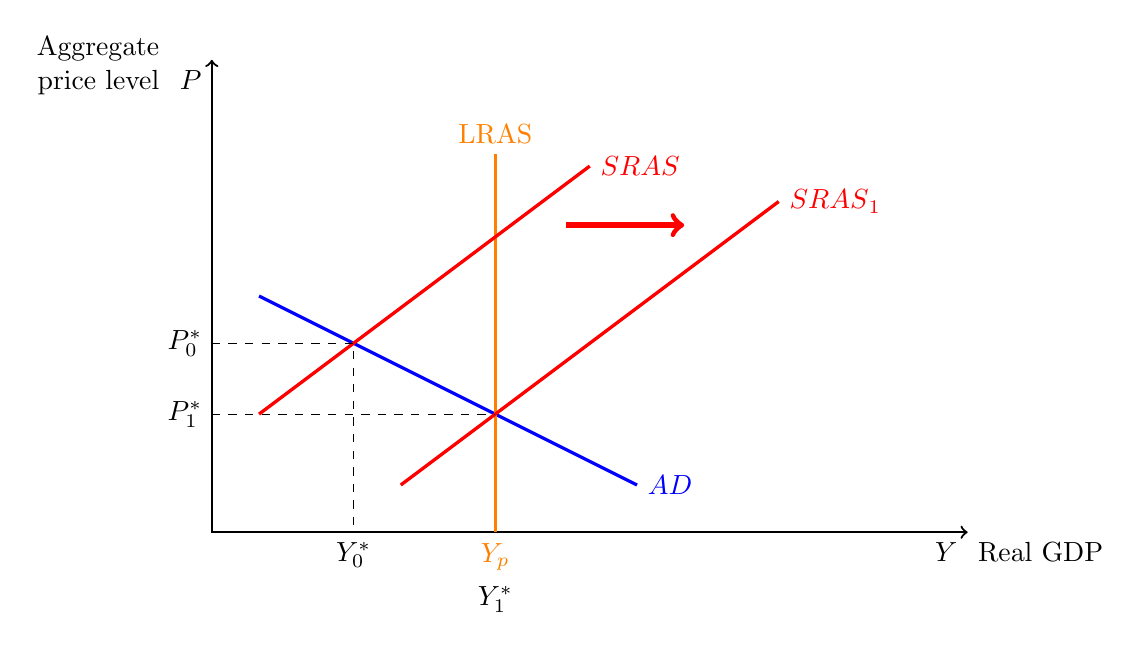
\begin{tikzpicture}[scale=0.6]
\draw[thick,<->] (0,10) node[below left,label={[align=right]left:Aggregate\\price level\\ }] {$P$} --(0,0)--(16,0) node[below left,label=right:Real GDP]{$Y$};
\draw[very thick,blue] (1,5)--(9,1) node[right]{$\text{AD}$};
\draw[very thick,orange] (6,0) node[below]{$Y_p$}--(6,8) node[above]{LRAS};
\draw[very thick,red] (1,2.5)--(8,7.75) node[right]{$\text{SRAS}$};
\draw[very thick,red] (4,1)--(12,7) node[right]{$\text{SRAS}_1$};
\draw[dashed] (0,4) node[left]{$P^*_0$} --(3,4) --(3,0)node[below]{$Y^*_0$};
\draw[dashed] (0,2.5) node[left]{$P^*_1$}--(6,2.5);
\node[below,yshift=-16pt] at (6,0) {$Y^*_1$};
\draw[line width=2pt,->,red] (7.5,6.5)--(10,6.5);
\end{tikzpicture}

A decrease in nominal wages causes an outward shift of the SRAS curve. (When labor is less expensive, firms will increase their output at any given price.)

As a result, prices decrease (from $P^*_0$ to $P^*_1$) and output increases (from $Y^*_0$ to $Y^*_1$).
\end{solution}

\item How does each variable change as an expansionary economy returns to long-run equilibrium?

\begin{solution}
\emph{Complete answer:} Nominal wages increase, the aggregate price level increases, and output decreases.

Here is a depiction of an expansionary economy:

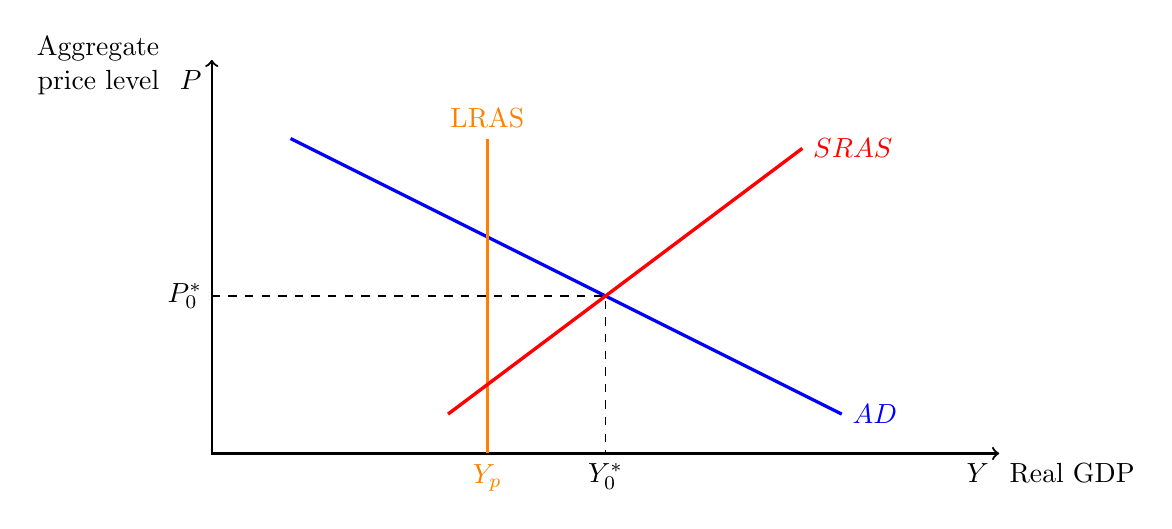
\begin{tikzpicture}[scale=0.5]
\draw[thick,<->] (0,10) node[below left,label={[align=right]left:Aggregate\\price level\\ }] {$P$} --(0,0)--(20,0) node[below left,label=right:Real GDP]{$Y$};
\draw[very thick,blue] (2,8)--(16,1) node[right]{$\text{AD}$};
\draw[very thick,orange] (7,0) node[below]{$Y_p$}--(7,8) node[above]{LRAS};
\draw[very thick,red] (6,1)--(15,7.75) node[right]{$\text{SRAS}$};
\draw[dashed] (0,4) node[left]{$P^*_0$} --(10,4) --(10,0)node[below]{$Y^*_0$};
\end{tikzpicture}

Output $Y^*_0$ is greater than potential output, $Y_p$. This solely defines an expansionary economy.

To return to long-run equilibrium, nominal wages adjust, shifting SRAS so that the output level returns to $Y_p$. We clearly need the SRAS curve to shift \emph{in} to return output to $Y_p$.

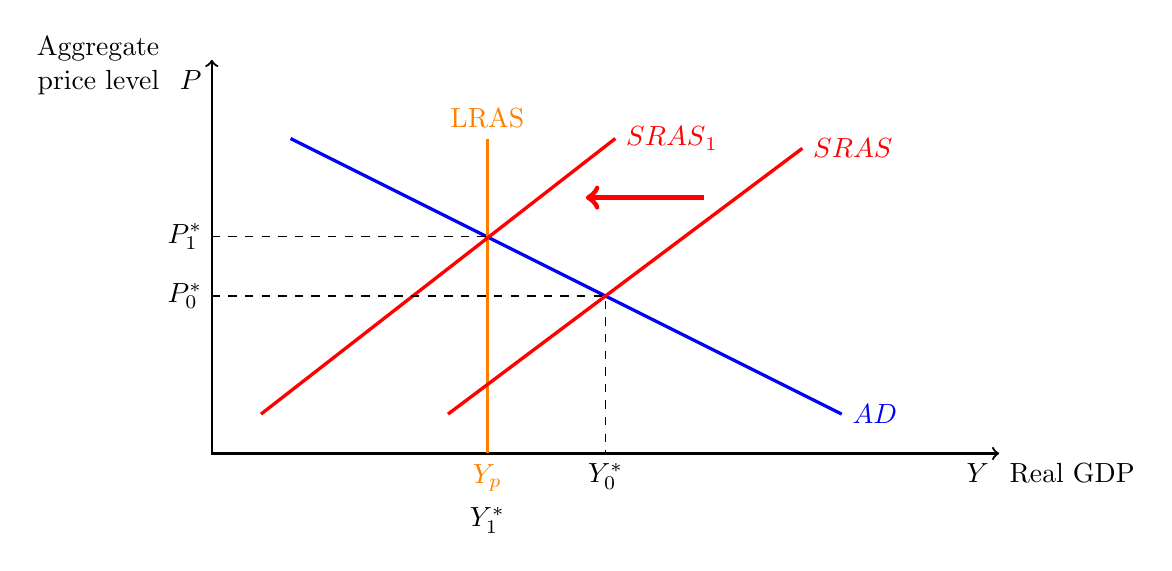
\begin{tikzpicture}[scale=0.5]
\draw[thick,<->] (0,10) node[below left,label={[align=right]left:Aggregate\\price level\\ }] {$P$} --(0,0)--(20,0) node[below left,label=right:Real GDP]{$Y$};
\draw[very thick,blue] (2,8)--(16,1) node[right]{$\text{AD}$};
\draw[very thick,orange] (7,0) node[below]{$Y_p$}--(7,8) node[above]{LRAS};
\draw[very thick,red] (6,1)--(15,7.75) node[right]{$\text{SRAS}$};
\draw[very thick,red] (1.25,1)--(10.25,8) node[right]{$\text{SRAS}_1$};
\draw[dashed] (0,4) node[left]{$P^*_0$} --(10,4) --(10,0)node[below]{$Y^*_0$};
\draw[dashed] (0,5.5) node[left]{$P^*_1$}--(7,5.5);
\node[below,yshift=-16pt] at (7,0) {$Y^*_1$};
\draw[line width=2pt,->,red] (12.5,6.5)--(9.5,6.5);
\end{tikzpicture}

An increase in nominal wages causes an inward shift of the SRAS curve. (When labor is more expensive, firms will reduce their output at any given price.)

As a result, prices increase (from $P^*_0$ to $P^*_1$) and output decreases (from $Y^*_0$ to $Y^*_1$).
\end{solution}

\end{enumerate}

\section{The U.S.~economy}

Please present a model of the U.S.~economy that relates output to an aggregate price level.

\begin{enumerate}

\item Please graph the economy in long-run equilibrium. Mark all curves with subscript ``0'' as well as output ($Y^*_0$) and price level ($P^*_0$). Be sure to also show potential output, $Y_p$, on your graph.

\begin{solution}

\begin{tikzpicture}[scale=0.5]
\draw[thick,<->] (0,10) node[below left,label={[align=right]left:Aggregate\\price level\\ }] {$P$} --(0,0)--(20,0) node[below left,label=right:Real GDP]{$Y$};
\draw[dashed] (0,1.75) node[left]{$P^*_0$}--(7,1.75);
\draw[very thick,blue] (2,4.25)--(8.5,1) node[right]{\contour{white}{$\text{AD}_0$}};
\draw[very thick,orange] (7,0) node[below]{$Y_p$}--(7,8) node[above]{LRAS};
\draw[very thick,red] (6,1)--(15,7.75) node[right]{$\text{SRAS}_0$};
\node[below,yshift=-16pt] at (7,0) {$Y^*_0$};
\end{tikzpicture}

\end{solution}

\end{enumerate}

Congress suddenly increases defense spending dramatically.

\begin{enumerate}[resume]

\item On your graph above, please draw this shock, labeling new curves with subscript ``1,'' the new output level as $Y^*_1$, and the new price level as $P^*_1$.

\begin{solution}

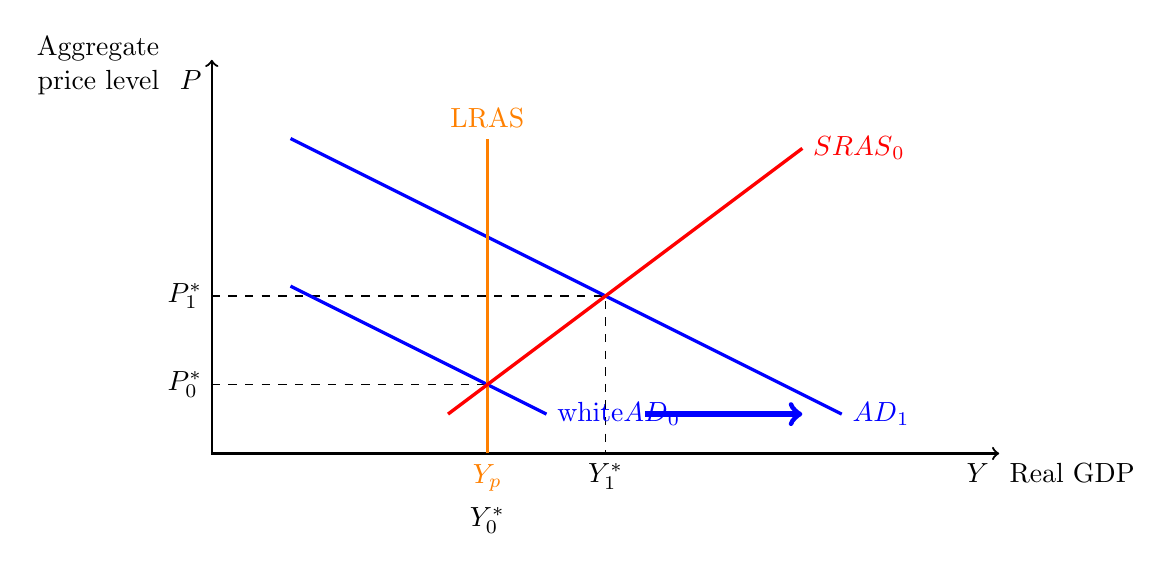
\begin{tikzpicture}[scale=0.5]
\draw[thick,<->] (0,10) node[below left,label={[align=right]left:Aggregate\\price level\\ }] {$P$} --(0,0)--(20,0) node[below left,label=right:Real GDP]{$Y$};
\draw[dashed] (0,1.75) node[left]{$P^*_0$}--(7,1.75);
\draw[dashed] (0,4) node[left]{$P^*_1$} --(10,4) --(10,0)node[below]{$Y^*_1$};
\draw[very thick,blue] (2,4.25)--(8.5,1) node[right]{\contour{white}{$\text{AD}_0$}};
\draw[very thick,blue] (2,8)--(16,1) node[right]{$\text{AD}_1$};
\draw[very thick,orange] (7,0) node[below]{$Y_p$}--(7,8) node[above]{LRAS};
\draw[very thick,red] (6,1)--(15,7.75) node[right]{$\text{SRAS}_0$};
\node[below,yshift=-16pt] at (7,0) {$Y^*_0$};
\draw[line width=2pt,->,blue] (11,1)--(15,1);
\end{tikzpicture}

\end{solution}

\item Is $Y^*_1$ above, below, or equal to potential output?

\begin{solution}
Above.
\end{solution}

\end{enumerate}

Over the subsequent years, the economy returns to long-run equilibrium.

\begin{enumerate}[resume]

\item Please depict this change on your graph, labeling new curves with subscript ``2,'' the new output level as $Y^*_2$, and the new price level as $P^*_2$.

\begin{solution}

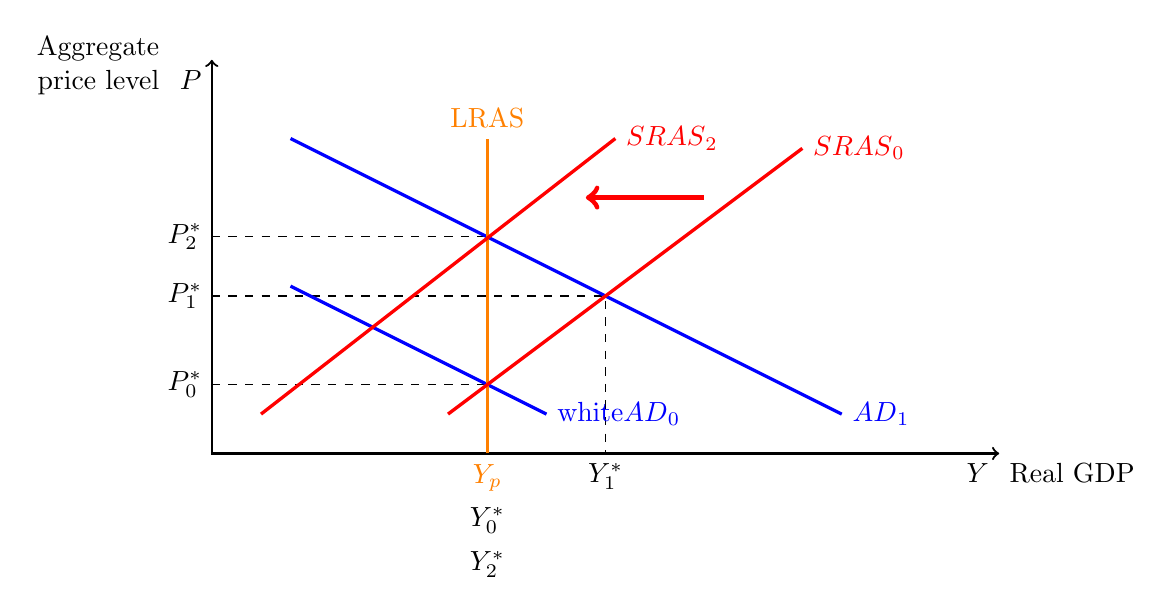
\begin{tikzpicture}[scale=0.5]
\draw[thick,<->] (0,10) node[below left,label={[align=right]left:Aggregate\\price level\\ }] {$P$} --(0,0)--(20,0) node[below left,label=right:Real GDP]{$Y$};
\draw[dashed] (0,1.75) node[left]{$P^*_0$}--(7,1.75);
\draw[dashed] (0,4) node[left]{$P^*_1$} --(10,4) --(10,0)node[below]{$Y^*_1$};
\draw[dashed] (0,5.5) node[left]{$P^*_2$}--(7,5.5);
\draw[very thick,blue] (2,4.25)--(8.5,1) node[right]{\contour{white}{$\text{AD}_0$}};
\draw[very thick,blue] (2,8)--(16,1) node[right]{$\text{AD}_1$};
\draw[very thick,orange] (7,0) node[below]{$Y_p$}--(7,8) node[above]{LRAS};
\draw[very thick,red] (6,1)--(15,7.75) node[right]{$\text{SRAS}_0$};
\draw[very thick,red] (1.25,1)--(10.25,8) node[right]{$\text{SRAS}_2$};
\node[below,yshift=-16pt] at (7,0) {$Y^*_0$};
\node[below,yshift=-32pt] at (7,0) {$Y^*_2$};
\draw[line width=2pt,->,red] (12.5,6.5)--(9.5,6.5);
\end{tikzpicture}

\end{solution}

\item Is $Y^*_2$ above, below, or equal to potential output?

\begin{solution}
Equal to.
\end{solution}

\end{enumerate}


\end{document}
